% -*- coding: utf-8 -*-

\section{Results}
\label{results}
\subsection{Introduction}
In this section I will discuss the results of the project. I will start by discussing the speed of the implemented features, and then talk about volume.

\subsection{Implemented features}
I have successfully implemented the RSS data-structure as well as its dependent class, a rectangle in 3D. 

Furthermore I have implemented all the required methods for the 2 classes.

\subsection{Comparisons}

In order to argue whether the quality of my implementation, I have tried to compare it with several other implementations - namely LSS' and OBBs. The parameters for comparison have been the volume of the data-structure, and the wall clock time required to check whether 2 BV overlaps or not.

\subsubsection{Generation of tests results}
All of the test results have been made by generating 2 arrays of
1000 random sets of points each - with 25 points in each set. I
maintain 2 arrays for each type of BV I create, with the intention of
checking each element from the first array against all elements in the
second array. This is done in order to ensure
that in practice a BV is never checked against itself, and also so
that I am quickly able to create large number of tests, without having
to use too much system memory. \\ 

For each point set in each array, I have created a 3 new BV's, one for
each of the types OBB, LSS, and RSS. Each BV contains the all points
in the pointset it was created from. Thus I create 2000 (split into 2 arrays of 1000 each)
new BV of each type. \\ 

I perform 2 test: 
\begin{description}
\item[Overlap:] I test the wall clock time required to perform the overlap test,
  for all 1.000.000 possible BV combinations, for all 3 types of BV. The creation of the BV's are as described above.  
\item[Volume:] I find the average volume of the individual BV's that cover a single point set, as well as the average of all possible BV combinations that can be created from combining 2 BV's.
\end{description}

All of these tests have been executed on a [my own computer specs].

\subsubsection{Overlap detection}

\begin{table}
\begin{tabular}{c|c|c|c|c}\\ 
& RSS: & RSS no-min & OBB: & LSS:\\ 
Total time spent: & 1,4220 & 1,4220 & 0,7030 & 0,1090\\ 
Number of overlaps: &1000000 & 1000000 & 1000000 & 1000000\\ 
\end{tabular}
\caption{\label{overlap-table}The table of the time used for the
  different overlaps checks. All of the times are in wall clock time seconds. The
  check reading ``RSS no-min'' is a RSS overlap check that is only run
with the axis separation test, and no minimum distance check first}
\end{table}

As it is clear from table \ref{overlap-table}, the current RSS overlap algorithm is slower than the one for both the OBB, and the LSS. 

This can partly be explained by the fact that, due to time constraints,
the overlap method for the RSS has not been optimized. But also the volumes of the RSS', which I will go into detail about below.

\subsubsection{Volume}
\label{volume-label}
\begin{table}
\begin{tabular}{c|c|c}\\ 
RSS average & OBB average & LSS average\\ 
3,246 & 1,081 & 1,176\\ 
\hline 
Combined RSS average & Combined OBB average & Combined LSS average\\ 
2,891 & 3,360 & 1,443\\ 
\end{tabular}
\caption{\label{volume-table} The average volume needed by the
  different BV to contain the points. The first row of values are the average
  volumes for each of the 2000 different BV that are produced, while
  the second row of values are the average volumes of the 1.000.000
  different combinations of BV's.}
\end{table}

\begin{figure}
\centering
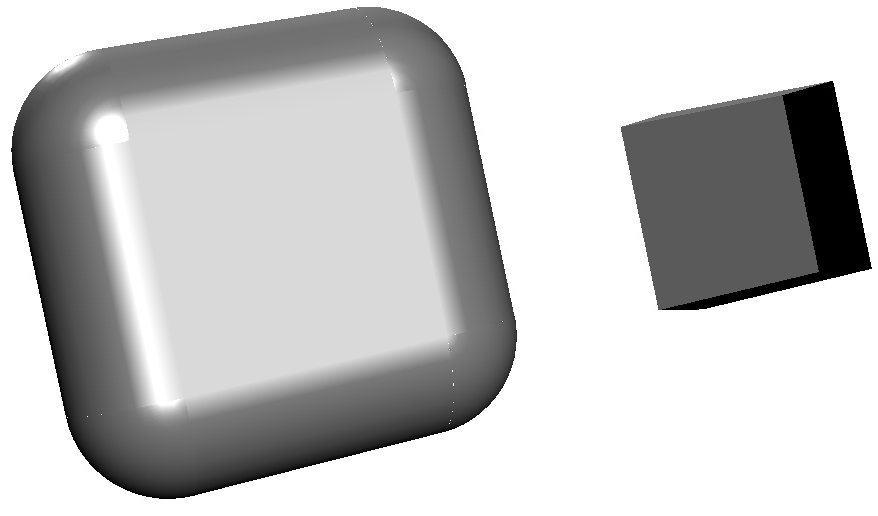
\includegraphics[width=0.5\textwidth]{figures/compareRSSOBB}
\caption{\label{compare-example}A RSS besides an OBB. The have been based on the same point-set, only transformed in the x dimension. It is clear that the RSS figure is larger than OBB}
\end{figure}

From table \ref{volume-table} it is clear that the current implementation of the RSS is worse than OBB's when it comes to a single point-set (this is also clear at figure \ref{compare-example}), but when it comes to combine 2 BV's, RSS outperforms OBB's, though not LSS'. 

\subsubsection{Problems with the current tests}
\label{test_problems}
All tests have been done on sets of points that have been generated randomly. It is therefore more likely that 2 BV's generated from the point sets are disjoint, than what would be the case in reality. This of course means that the results listed here can mainly be used to gauge how well the algorithms handle the cases where most of the point sets are disjoint.

It is worth mentioning, that as implemented, OBB's and RSS' both uses the Axis separation test, but as mentioned in \ref{overlap}, RSS first checks the minimum distance between the two RSS' is less than their combined radii. So everything else being equal, it is clear that the RSS overlap check would have to do more work than the worst case overlap test for OBB's. Since the current version of the RSS also has a greater average volume than the OBB (see \ref{volume-label}), RSS' should report more overlaps than OBB's, which in practice should give it a worse run time.
 
Furthermore, as described in \ref{implementation_axis_sep}, given 2 RSS' A and B, I have not made the axis go through A (which in practice would mean that I would have had to find the transformation of A so that it became axis-parallel, and then transforming both A and B so with the same transformation) \Sfixme{Better explanation or remove entirely?}. Since all OBB's in ProGAL are axis oriented, this is trivially true for its axis-separation test, with all the possible optimizations that enables.

\subsection{Conclusion}
I have in this section shown that the current implementation of the RSS performs worse than both the OBB and the LSS on both the metrics of volume and wall clock time when performing overlap detection. If the RS data-structure is to be used in practice, these limitations must be overcome.
